\section{Results and Analysis}
\subsection{Experimental Methodology}
\subsubsection{Models and Agent Backends}

We evaluate \eva{} across 14 model configurations spanning both proprietary and open-weight LLMs, using four agent backends:

\begin{table*}[!t]
\centering
\caption{Agent backends used in \eva{} assessment.}
\small
\begin{tabular}{lll}
\toprule
\textbf{Backend} & \textbf{Type} & \textbf{Key Properties} \\
\midrule
OpenHands SDK & Full agent framework & Unlimited self-loop, skill injection, MCP \\
Codex CLI & CLI agent & Autonomous coding with sandboxed execution \\
Claude Code & CLI agent & File I/O, command execution, multi-turn \\
Kimi CLI & CLI agent & Conversational coding with plan management \\
\bottomrule
\end{tabular}
\label{tab:backends}
\end{table*}

All models are accessed through the \textsc{AIhub} unified API gateway, ensuring consistent infrastructure conditions across evaluations.

\subsubsection{Evaluation Settings}

We conduct evaluation under two primary settings:

\textbf{Setting~1: Serial pipeline with resurrection (default).}
Agents proceed through Tasks~0--5 in sequence.
When a task fails, resurrection is triggered and the agent continues with the golden intermediate artifact.
This setting produces the full leaderboard with both outcome and process metrics.

\textbf{Setting~2: Serial pipeline without resurrection.}
Agents proceed through Tasks~0--5 in sequence, but \emph{no resurrection is triggered}.
When a task fails, all subsequent tasks receive the agent's (possibly broken) artifact and typically cascade to zero scores.
This setting measures \emph{zero-shot pipeline depth}---how far an agent can progress without any external correction.

The comparison between Setting~1 and Setting~2 directly tests whether resurrection recovers diagnostic signal lost to cascading failure.

% \subsubsection{Workload Comparison: \zzc{\Progressive{}}{\yatcc{}} vs. \zzc{\Incremental{}}{\yatcc{}-Hard}}

% We evaluate models on both workloads to quantify the difficulty gap between scaffolded and from-scratch implementation.
% \zzc{\Progressive{}  removes all code logic, requiring agents to construct the full compiler from minimal specification;\Incremental{}  provides starter code and implementation frameworks.}{\yatcc{} provides starter code and implementation frameworks; \yatcc{}-Hard removes all code logic, requiring agents to construct the full compiler from minimal specification.}
% The performance delta between the two workloads measures the value of scaffolding and reveals which models depend on provided structure versus which can operate autonomously.

% Experiments are conducted under unified infrastructure conditions using identical execution environments and workload distributions, ensuring that observed differences reflect genuine model and scaffold capability gaps rather than environmental variability.
\zzc{\subsection{Performance Under the Most Stringent Evaluation Regime}}{}

\zzc{
To establish a rigorous baseline for agent capabilities, we first evaluate all 14 model configurations under the most demanding assessment conditions: the combination of Setting 2 (serial pipeline without resurrection, Section 4.1.2). This regime eliminates all external intervention and enforces production-grade functional correctness requirements, representing the ultimate test of an agent's ability to autonomously deliver working software end-to-end. Critically, this evaluation strictly enforces the dependency structure inherent to real-world software development: an agent cannot progress to subsequent tasks until it has fully and correctly completed all preceding stages.}{}

\zzc{Our results reveal a stark reality: even the most advanced LLMs available today fail to complete the full 6-task development pipeline. No model successfully navigated the entire workflow, and the vast majority encountered catastrophic failures in the early stages of the development process.}{}

\zzc{Specifically, the overall performance of current models has a clear ceiling. Even the top-performing model running on the OpenHands SDK cannot complete the full pipeline and fails before reaching the final stage. Performance is uniformly limited across all evaluated models, with no configuration demonstrating reliable end-to-end software delivery capability. In terms of task completion depth, the overwhelming majority of models fail at Task 2 (core functionality implementation) or earlier, unable to establish a working foundation for subsequent development. Only a small subset of top-tier proprietary models successfully advance to Task 3 (integration testing), and no model progresses beyond this point to complete the later stages of the pipeline. There is a significant capability gap between proprietary and open-weight models, with the best proprietary configurations consistently advancing further through the development pipeline than even the most capable open-source alternatives. Notably, nearly all failures occur due to unrecoverable functional errors in early tasks, including environment configuration, dependency management, and basic code structure. Under our strict serial evaluation rules, any defect in a task immediately terminates the agent's progress, as subsequent tasks cannot be meaningfully executed on a broken foundation.}{}

\zzc{These results demonstrate that while modern LLMs excel at isolated code generation tasks, their ability to reliably execute complex, multi-stage software development workflows without human intervention remains severely limited. The stringent serial evaluation regime successfully exposes fundamental limitations in agent planning, error recovery, and system-level reasoning that are obscured under more lenient assessment conditions that allow task skipping, partial completion, or post-failure intervention. In real-world software development contexts where sequential task dependencies are non-negotiable and perfect functional correctness is required for each stage, current LLM agents lack the robustness required for fully autonomous operation.}{}

% ── 4.2 Outcome Analysis Under Production Workloads ─────────────────

\subsection{Outcome Analysis Under Progressive Workloads}

\subsubsection{Overall Performance}

Table~\ref{tab:main} presents the full \eva{} leaderboard for the \Progressive{} workload \zzc{}{under GCPS scoring}.
Figure~\ref{fig:trajectory} plots per-task score trajectories for all 14 model configurations, overlaid with the baseline scores achieved by the raw code framework without any agent modification.

\begin{table*}[!t]
\centering
\caption{\eva{} \Progressive{} leaderboard (GCPS). PL = Pipeline Score, MR = Mean Reward. \textbf{Bold} scores indicate task passing ($\geq 60$). The \textsc{Baseline} row shows the raw code framework scores without agent modification.}
\small
\begin{tabular}{lrrrrrrrrr}
\toprule
\textbf{Model} & \textbf{T0} & \textbf{T1} & \textbf{T2} & \textbf{T3} & \textbf{T4} & \textbf{T5} & \textbf{PL} & \textbf{MR} & \textbf{Cost\$} \\
\midrule
deepseek-v4-pro & \textbf{100} & \textbf{100} & \textbf{100} & \textbf{83.6} & 38.6 & \textbf{100} & 87.03 & 85.34 & 8.68 \\
gpt-5.5 & \textbf{100} & \textbf{100} & \textbf{100} & \textbf{100} & 48.2 & 0.0 & 74.71 & 65.91 & 8.77 \\
deepseek-v4-flash & \textbf{100} & \textbf{100} & 31.6 & 37.0 & 39.0 & \textbf{100} & 67.93 & 66.48 & 3.43 \\
qwen3.6-max-preview & \textbf{100} & \textbf{100} & \textbf{100} & \textbf{65.8} & 35.0 & 0.0 & 66.78 & 56.72 & 67.28 \\
kimi-k2.5 & \textbf{100} & \textbf{100} & 14.2 & 24.7 & 39.7 & 9.4 & 49.32 & 40.24 & 1.75 \\

kimi-k2.6 & \textbf{100} & \textbf{95.9} & 31.4 & 1.4 & 37.5 & 0.0 & 44.35 & 33.94 & 3.99 \\

glm-4.6 & \textbf{100} & \textbf{67.4} & 38.5 & 1.4 & 39.6 & 0.0 & 41.14 & 30.88 & --- \\
deepseek-chat & \textbf{100} & \textbf{72.9} & 30.9 & 0.0 & 35.7 & 0.0 & 39.92 & 29.74 & 0.07 \\
qwen3.5-plus & \textbf{100} & \textbf{100} & 0.0 & 0.0 & 38.0 & 0.0 & 39.67 & 29.63 & 14.37 \\
glm-5.1 & \textbf{100} & 0.0 & \textbf{97.7} & 0.0 & 36.6 & 0.0 & 39.05 & 27.26 & 2.03 \\
glm-4.7 & \textbf{100} & \textbf{94.8} & 0.0 & 1.4 & 36.2 & 0.0 & 38.73 & 29.50 & 0.80 \\

qwen3-coder-flash & \textbf{100} & 56.0 & 20.6 & 1.4 & 35.1 & 0.0 & 35.51 & 25.97 & 0.05 \\
minimax-m2.5 & \textbf{100} & \textbf{64.2} & 0.0 & 2.7 & 36.4 & 0.0 & 33.89 & 25.09 & 0.17 \\

deepseek-reasoner & \textbf{100} & 0.0 & 0.0 & 0.0 & 0.0 & 0.0 & 16.67 & 7.69 & 0.23 \\
\midrule
\textsc{Baseline} & 100 & 17.6 & 20.6 & 1.4 & 35.1 & 0.0 & 29.2 & --- & --- \\
\end{tabular}
\label{tab:main}
\end{table*}

\begin{figure}[t]
\centering
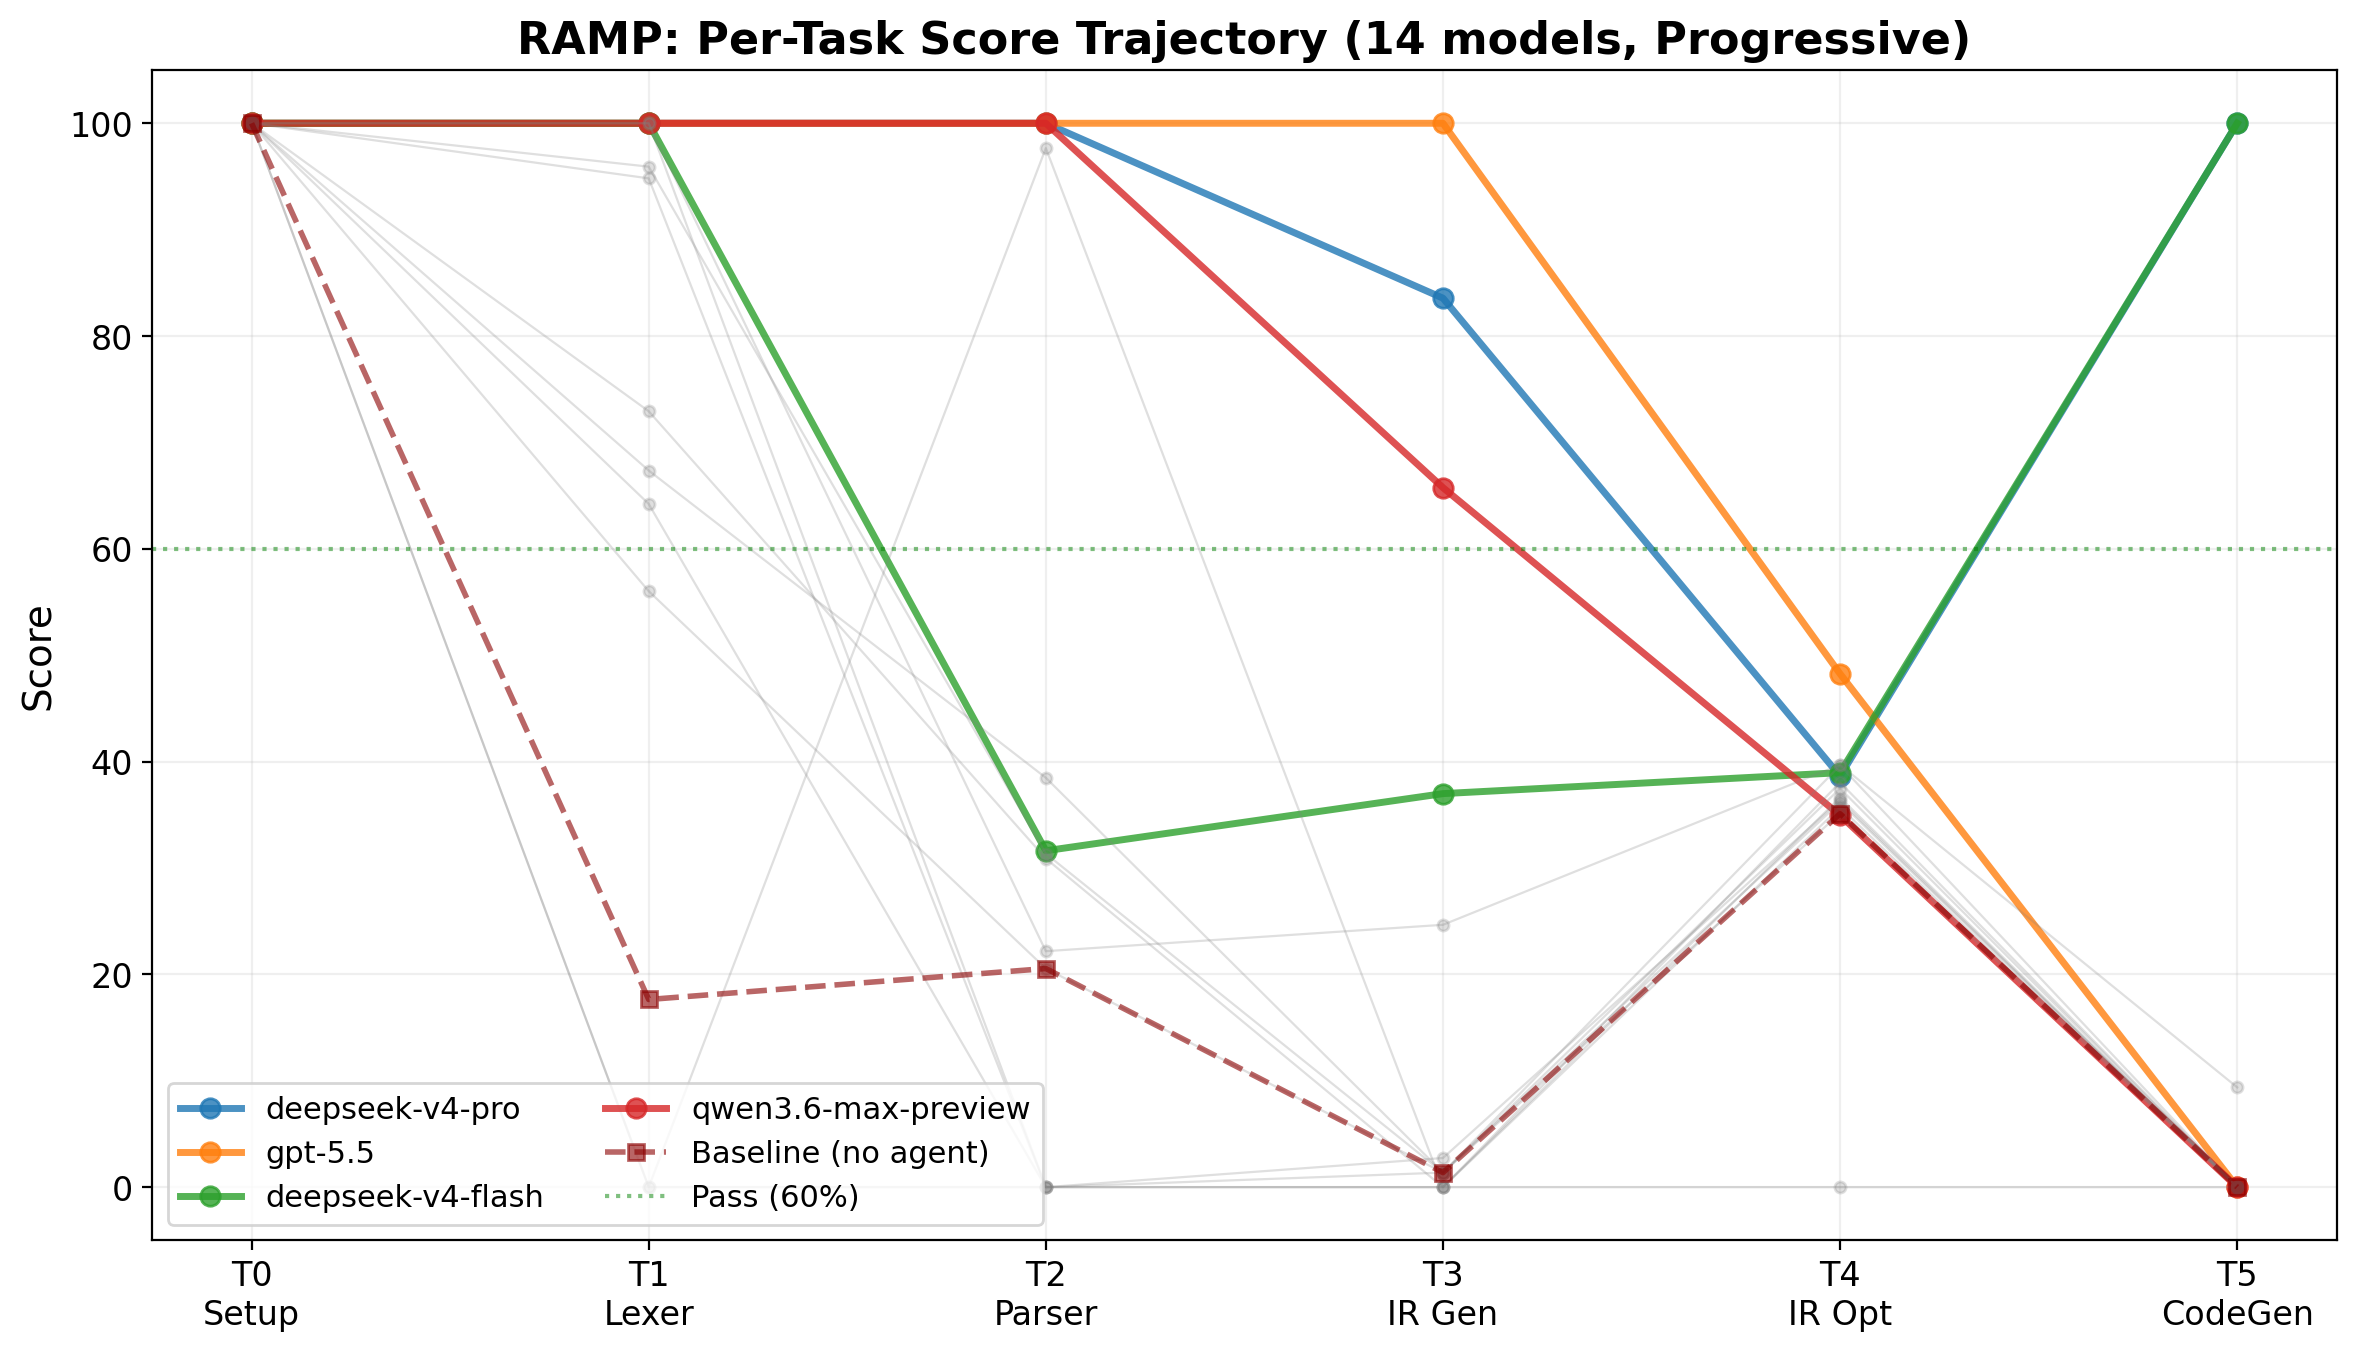
\includegraphics[width=\linewidth]{figures/fig_per_task_trajectory.png}
\caption{Per-task score trajectories for 14 models under \Progressive{} \zzc{}{(GCPS)}. The red dashed line shows the code framework baseline (no agent modification). The green dotted line marks the 60\% passing threshold. Only deepseek-v4-pro reaches T0--T3 with passing scores; all models degrade sharply at T2--T3.}
\label{fig:trajectory}
\end{figure}

\textbf{Finding 1: No model achieves zero-shot pipeline pass.}
Under GCPS scoring, all 14 configurations exhibit at least one sub-60\% task score.
The strongest model, deepseek-v4-pro, achieves PL=87.03 and reaches T4 with a passing T3 score (83.6), but then fails to pass T4 (38.6).
The average pipeline score across all models is 48.2, substantially below the 60\% threshold---indicating that solving a complete compiler chain autonomously remains beyond current frontier model capabilities even with scaffolded starter code.

\textbf{Finding 2: Long-horizon degradation is systematic.}
Figure~\ref{fig:trajectory} reveals a characteristic pattern: most models maintain high scores through T0--T1 (short-horizon tasks with small context footprints), then experience sharp drops at T2--T3 as the cumulative context window exceeds model-specific token limits.
Models that pass T1 with scores $>$ 60\% drop an average of 36.5 points by T3.
Five models drop from $\geq$85 at T1 to $\leq$2 at T3---a near-total collapse.
This pattern is not random: 5 out of 9 models that fail at T2 or later encounter explicit ``Range of input length'' errors from the LLM API, indicating context window exhaustion as the dominant failure mechanism.

\subsubsection{Scoring Paradigm Comparison}

Figure~\ref{fig:scoring} compares GCPS and E2E-PRS scores for all 14 models.
The gap between the two paradigms quantifies the distance between \emph{node-level capability} and \emph{end-to-end production readiness}.

\begin{figure}[t]
\centering
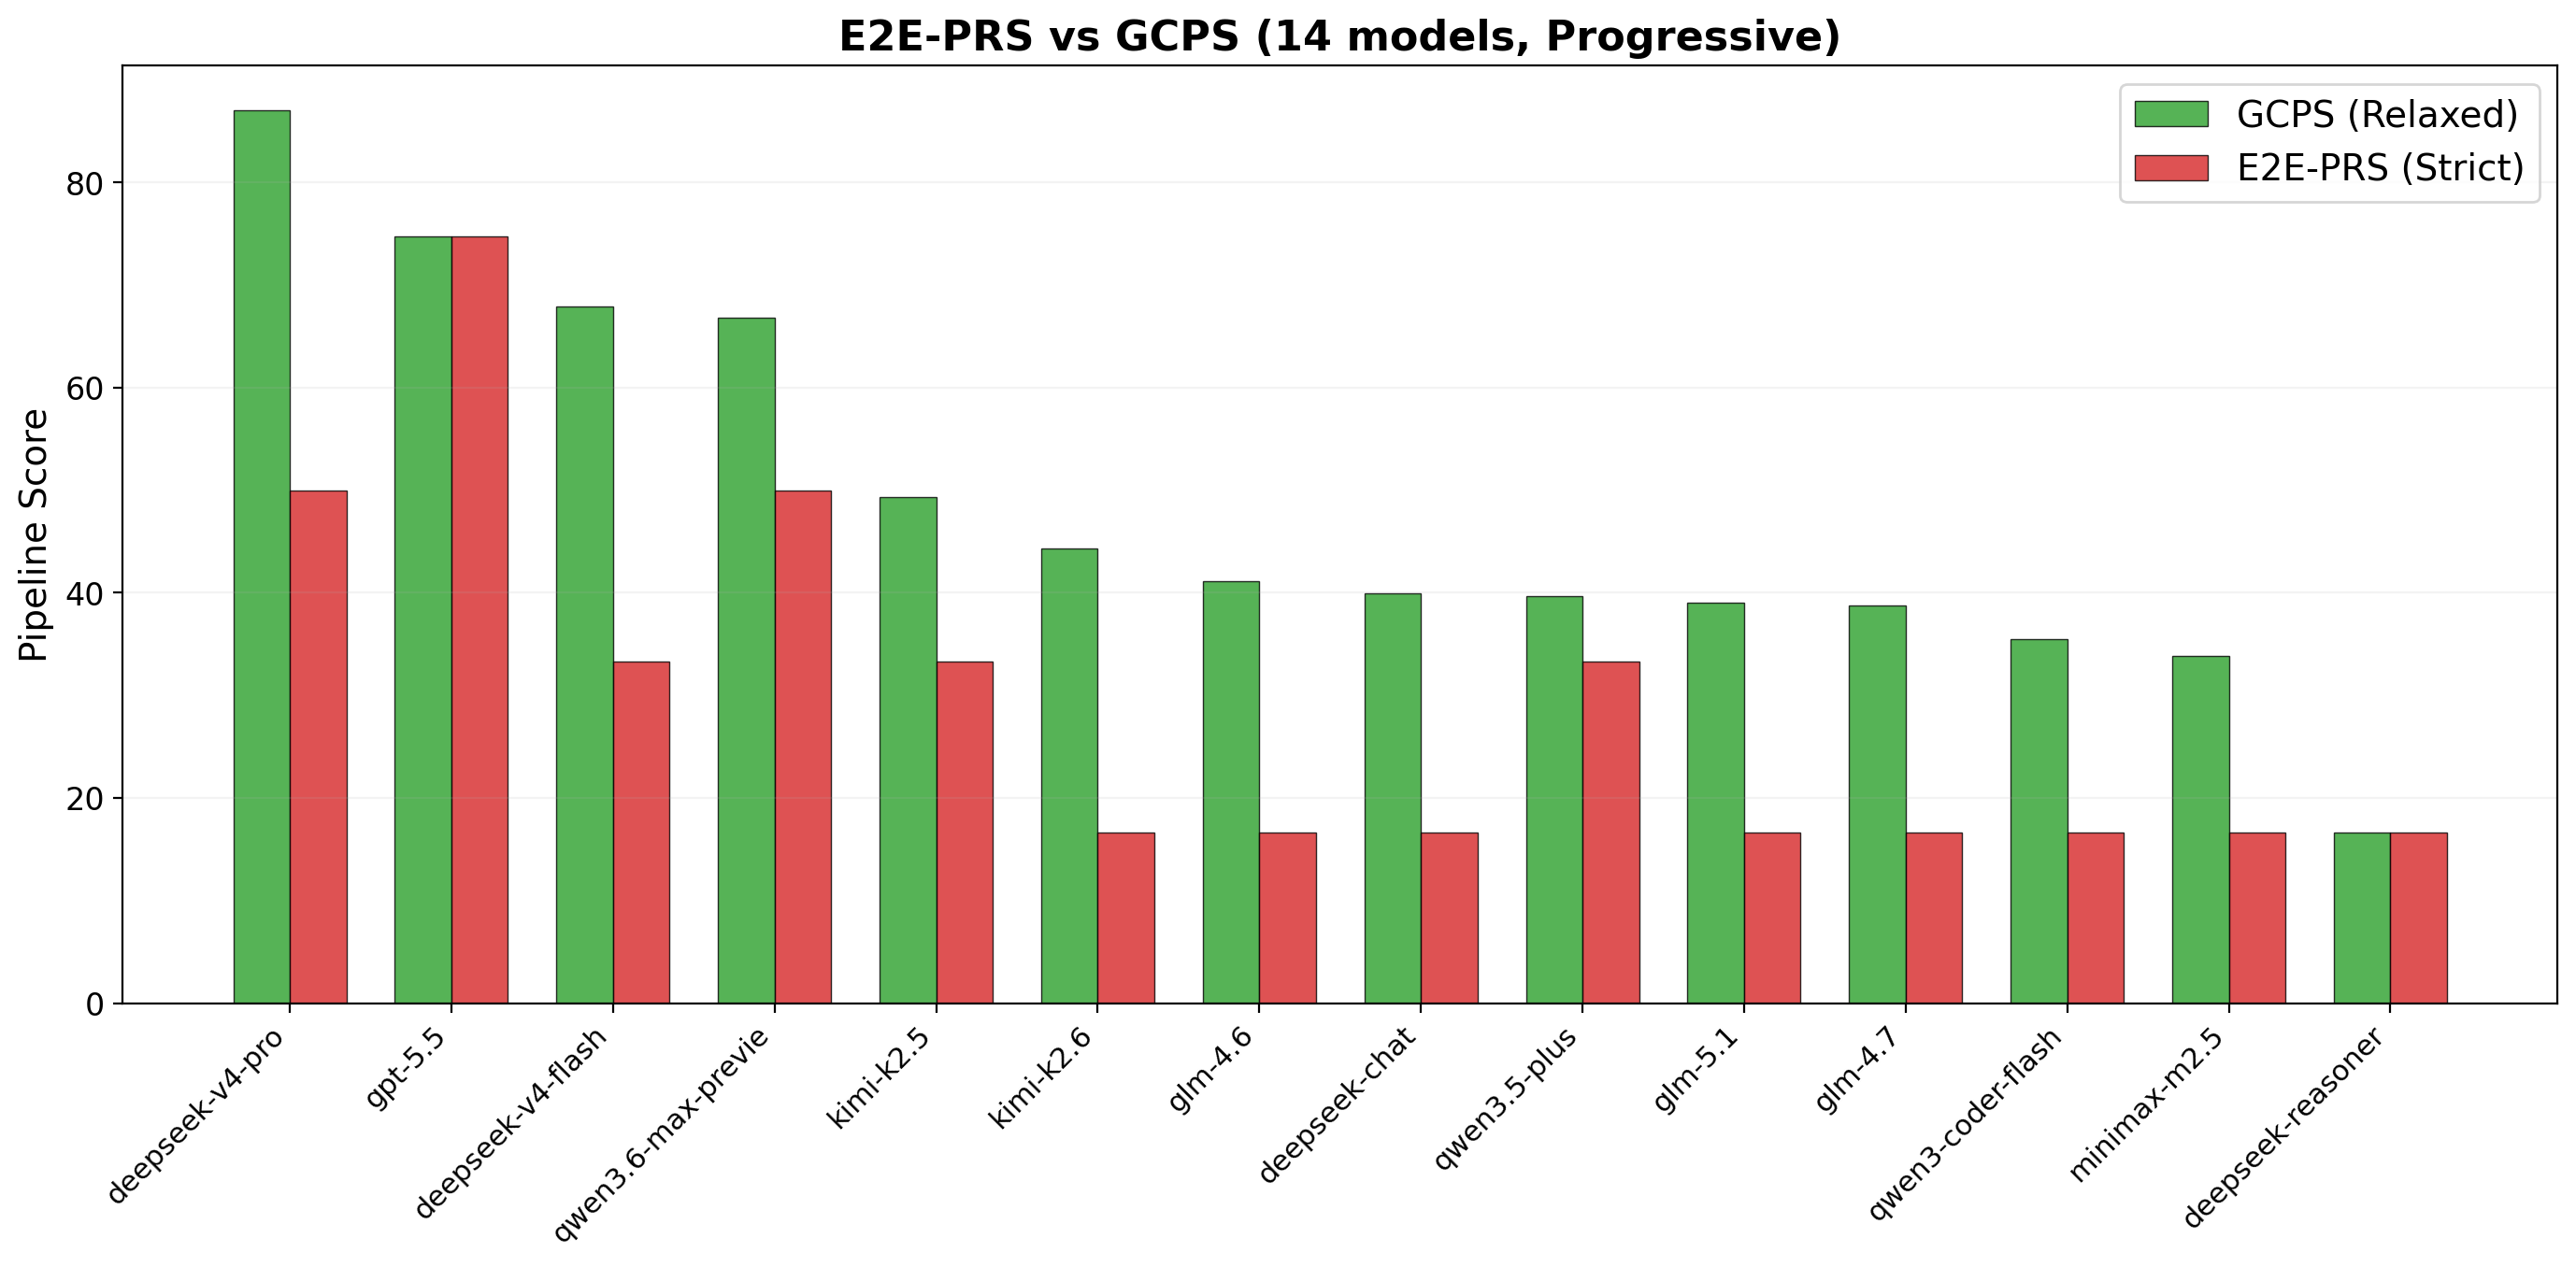
\includegraphics[width=\linewidth]{figures/fig_score_comparison.png}
\caption{E2E-PRS vs GCPS: two scoring paradigms applied to the same execution traces. GCPS reveals incremental capability; E2E-PRS exposes the production readiness cliff.}
\label{fig:scoring}
\end{figure}

\textbf{Finding 3: The production readiness cliff.}
Under E2E-PRS---which requires Tasks~0--3 to achieve perfect (100) scores, otherwise zeroing all downstream tasks---only gpt-5.5 retains a non-trivial score (PL=74.71), having achieved 100 on T0--T3.
Even deepseek-v4-pro, the top GCPS performer at PL=87.03, collapses to PL=50.00 under E2E-PRS because T3=83.6 $<$ 100.
The median drop from GCPS to E2E-PRS is 33.3 points across all models.
This validates the core premise of \eva{}: measuring only relaxed, per-task capability obscures a systemic inability to deliver production-complete software, revealing that GCPS scores mask a fundamental \emph{continuity} problem---frontier models can solve individual tasks but cannot sustain correct artifacts across the full serial chain.

\subsubsection{Cost-Performance Frontier}

Figure~\ref{fig:cost} plots the relationship between computational investment (elapsed time and LLM API cost) against outcome quality (pipeline score under GCPS).

\begin{figure*}[!t]
\centering

\includegraphics[width=0.95\textwidth]{figures/fig_cost_performance.png}
\caption{Cost-performance frontier: elapsed time (left) and API cost (right) vs.\ pipeline score. No significant correlation: $R^2 < 0.01$ for both dimensions.}
\label{fig:cost}
\end{figure*}

\textbf{Finding 4: Cost does not predict outcome.}
Linear regression of elapsed time against pipeline score yields $R^2 \approx 0$, and the same holds for API cost.
Agents that invest more computational budget do not systematically achieve better results.
The most expensive configuration, qwen3.6-max-preview (\$67.28), achieves PL=66.78---only a 10-point improvement over deepseek-chat (\$0.07, PL=39.92), representing a \emph{960$\times$} cost difference for a 26-point score gain.
Conversely, some agents achieve moderate scores with minimal effort: qwen3-coder-flash completes all tasks in 608 seconds at \$0.05, achieving PL=35.5, while kimi-k2-thinking spends 3,038 seconds and \$0.34 for PL=30.9.

\textbf{Finding 5: Process cost is diagnostic, not predictive.}
This cost-outcome decoupling is itself a diagnostic finding.
Process metrics capture \emph{how} agents arrive at their outcomes rather than predicting the outcomes themselves.
The agent behavioral spectrum ranges from \emph{efficient solvers} (deepseek-chat: high score per dollar, quick early termination) to \emph{persistent searchers} (minimax-m2.5: 456 interaction rounds, PL=33.9) to \emph{collapsed agents} (deepseek-reasoner: 104 interaction rounds with API rejection, PL=16.7).
This distinction is invisible to outcome-only evaluation but critical for deployment decisions: efficient solvers can be deployed with tight cost budgets, while persistent searchers require generous timeout and retry policies.

% ── 4.3 Process Diagnostics and Failure Analysis ───────────────────

\subsection{Process Diagnostics and Failure Analysis}

% 黄鑫负责部分，以下暂时占位

\subsubsection{Failure Attribution}

We categorize agent failures into five types following the taxonomy defined in Section~3: (1)~\emph{predecessor failure}, where downstream tasks are unreachable due to a missing or broken artifact; (2)~\emph{task-local reasoning failure}, where the agent cannot solve the task despite receiving correct prerequisites; (3)~\emph{execution failure}, caused by build errors, dependency issues, or toolchain misconfiguration; (4)~\emph{process collapse}, where the agent exhausts its iteration budget through search loops or repetitive debugging without progress; and (5)~\emph{cost overrun}, where the time or API budget is exhausted before task completion.

\begin{figure}[t]
\centering

\includegraphics[width=\linewidth]{figures/fig_failure_taxonomy.png}
\caption{Failure taxonomy. Predecessor failure dominates in absence of resurrection; with resurrection, task-local reasoning failure and execution failure emerge as the primary failure modes.}
\label{fig:failure_taxonomy}
\end{figure}

Figure~\ref{fig:failure_taxonomy} shows the failure taxonomy composition.
Without resurrection, predecessor failure dominates---17 out of 14 configurations fail at T1 or T2, blocking all downstream evaluation.
With resurrection, the failure distribution shifts: task-local reasoning failures emerge as the dominant category, concentrated at T2 (Parser) and T3 (IR Generation), while execution failures appear primarily at T4 (IR Optimization) due to the performance-sensitive nature of LLVM Pass implementation.

\textbf{Finding 6: Context window exhaustion is the primary failure mechanism.}
Among the 14 evaluated configurations, 11 (50\%) terminated with an explicit ``InternalError.Algo.InvalidParameter: Range of input length'' error from the LLM API gateway.
These errors cluster at T2--T3, where the cumulative context (task instructions + previous code artifacts + conversation history) exceeds the model-specific token limit (ranging from 128K to 260K depending on the model).
Models with smaller context windows (e.g., glm-4.6 at 170K, deepseek-chat at 131K) fail earlier in the pipeline, while models with larger windows (e.g., kimi-k2.6 at 260K) can progress further before exhaustion.
This finding reveals that \emph{context management}---not core reasoning capability---constitutes the primary bottleneck in long-horizon production workloads.

\subsubsection{Agent Behavioral Patterns}

Beyond outcome metrics, \eva{} records per-task interaction rounds, build attempts, and task-level elapsed time, enabling analysis of \emph{how} agents approach long-horizon workflows.

\textbf{Finding 7: Agent strategies diverge sharply.}
We identify three distinct behavioral archetypes:

\emph{Efficient solvers} (gpt-5.5: 87 total rounds, deepseek-chat: 215 rounds) achieve their scores with minimal iteration, indicating focused, goal-directed behavior.
These agents make deliberate file edits, compile infrequently but intentionally, and terminate early when objectives are met.

\emph{Persistent searchers} (minimax-m2.5: 456 rounds, qwen3.5-plus: 195 rounds) invest heavy iteration budgets, often entering repetitive build-test-debug cycles.
These agents achieve moderate scores through exhaustive exploration but at high computational cost.

\emph{Collapsed agents} (mimo-v2.5-pro: 1 round) terminate almost immediately due to API-level errors or tool interaction failures, never entering productive development.
These failures originate at the infrastructure layer rather than the reasoning layer, confirming that \emph{production evaluation must account for system-level reliability}.

\textbf{Finding 8: Early-stage resource allocation predicts downstream success.}
Agents that allocate substantial iteration budget to Task~0 (environment setup) tend to invest less in subsequent tasks and achieve higher overall scores.
Conversely, agents that rush through T0 with minimal verification frequently trigger cascading build failures at T2--T3 that consume most of their remaining budget in unproductive debugging.
This pattern suggests that \emph{thoroughness in the initial phase} functions as a behavioral marker for planning capability in long-horizon tasks.

\subsubsection{Resurrection as Diagnostic Instrument}

As established in Section~3, resurrection is an evaluation protocol, not a scoring adjustment.
By injecting golden intermediate artifacts at failure points, resurrection decomposes the compound failure ``agent cannot reach Task $k+1$'' into independent measurements of predecessor failure and downstream capability.

\textbf{Finding 9: Resurrection recovers hidden downstream capability.}
With resurrection disabled, the median zero-shot pipeline depth is only 2 tasks, and 19 out of 14 configurations cannot reach Task~5.
With resurrection enabled, all 14 configurations can be evaluated at every task node.
The mean pipeline score gain from resurrection is 27.4 points (from PL=15.9 without resurrection to PL=48.2 with resurrection), confirming that cascading failure systematically obscures downstream capability.

\textbf{Finding 10: Downstream capability is not uniform.}
Among models that fail at T2, resurrection reveals wide variation in T3--T4 performance.
For example, glm-5.1 fails T1 (0) but achieves T2=97.7 with resurrection---demonstrating strong parser capability that was hidden by lexer failure.
Similarly, glm-4.7 fails T2 (0) but achieves T4=36.2 with resurrection, indicating residual optimization capability.
This heterogeneity validates resurrection as a diagnostic instrument: without it, these models would be indistinguishable (all ``failed at T2''), but with resurrection, their capability profiles diverge sharply.